\centerline{\bf \Huge ГМТ}

\begin{flushright}
        \scriptsize{Ты поймёшь, как важно идти вперёд, как только сделаешь первый шаг.\\ Мисато Кацураги}
\end{flushright}

\begin{wrapfigure}{r}{0.6\linewidth}
    \vspace{-8mm}
    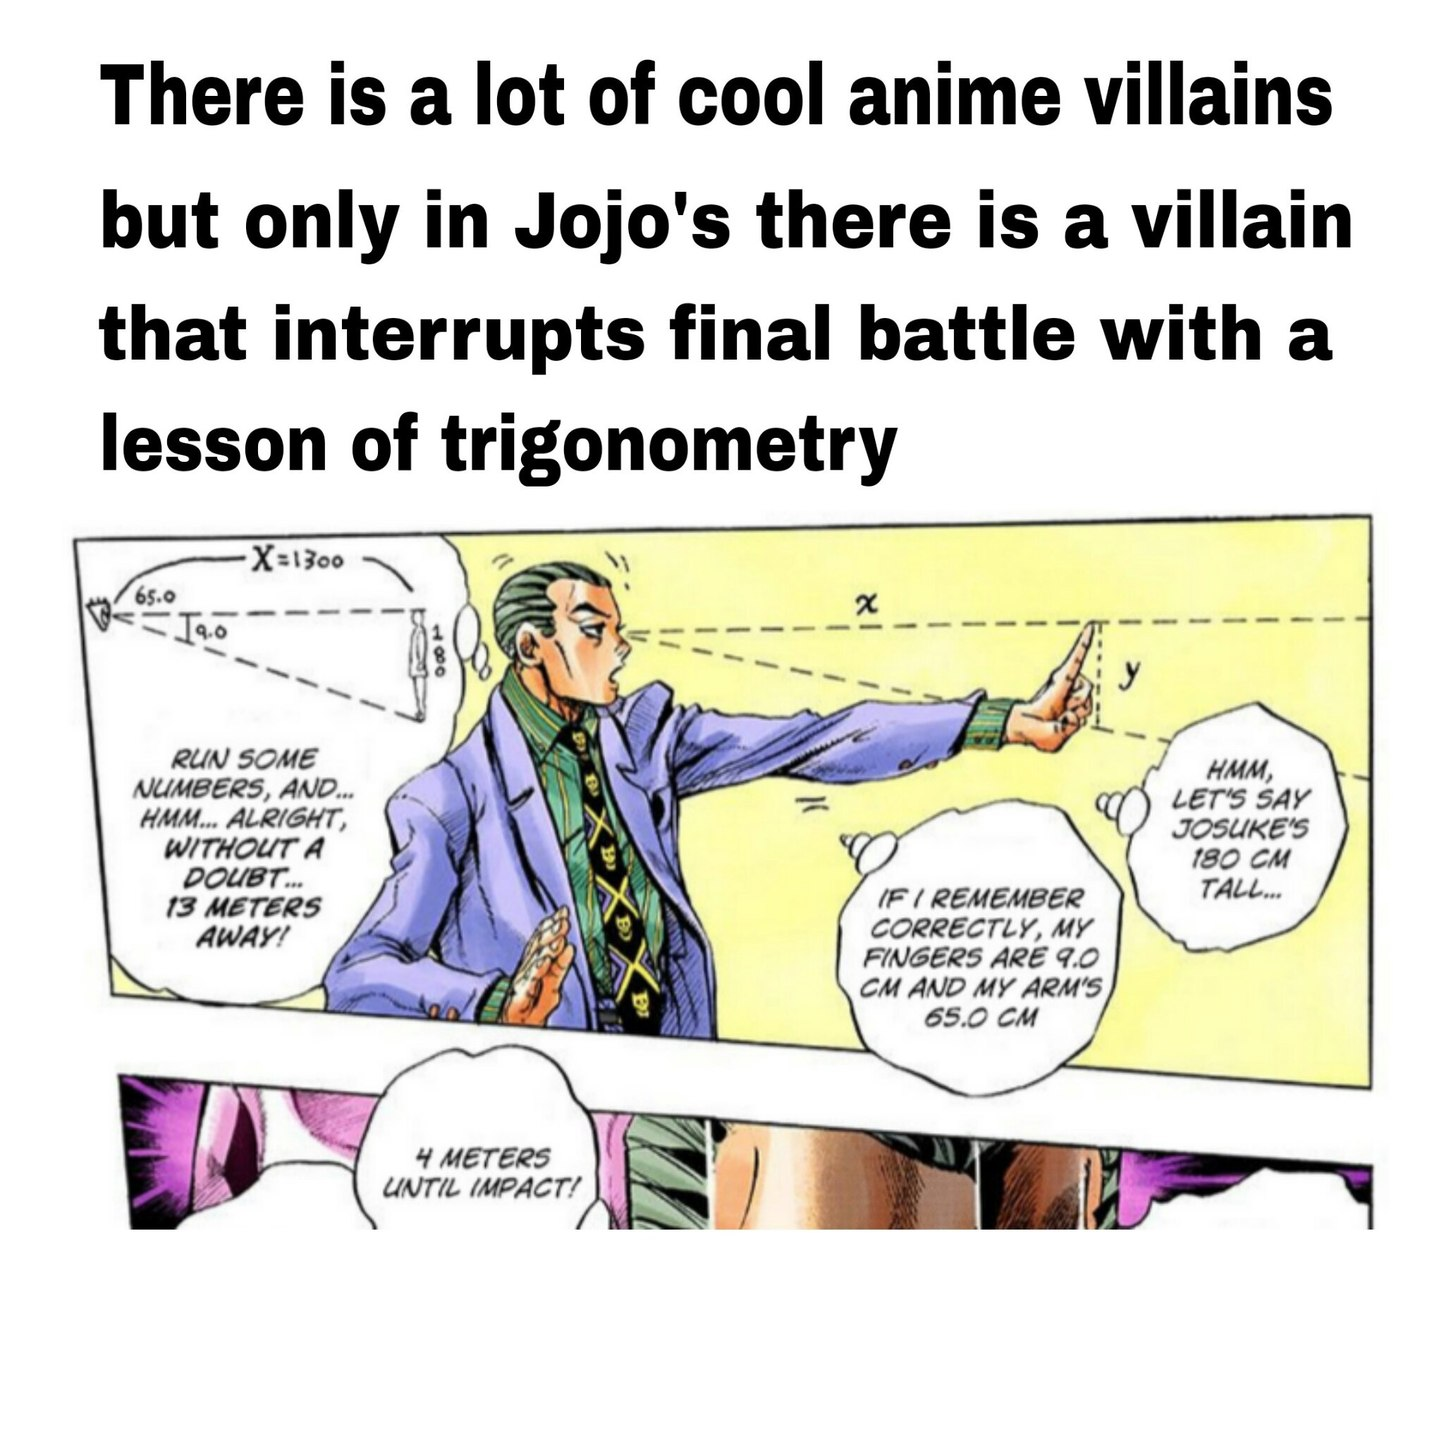
\includegraphics[width=\linewidth]{Матсфера. Ахмед/Летняя смена/7 класс/jojo.png}
\end{wrapfigure}

\par\noindent
\vspace{-8mm}

\textbf{Определение.} Геометрическое место точек (ГМТ), обладающих заданным свойством, --- это фигура, состоящая из тех и только тех точек, для которых это свойство выполняется.

Поэтому, найдя искомое ГМТ --- фигуру $F$, надо доказать два взаимно обратных утверждения:

1) Любая точка, принадлежащая $F$, обладает указанным свойством.

2) Любая точка, обладающая указанным свойством, принадлежит $F$.



\centerline{Простейшие ГМТ на плоскости.}

1) ГМТ, находящихся на данном расстоянии от данной точки ---

2) ГМТ, равноудаленных от двух данных точек ---

3) ГМТ, находящихся на данном расстоянии от данной прямой ---

4) ГМТ, равноудаленных от двух данных прямых (два случая) ---



\newpage

\hspace{3mm}

\problem{1}
Окружность радиуса R катится по прямой. По какой траектории движется ее центр?

\problem{2}
Дан отрезок $A B$. Найдите ГМТ $X$ таких, что: $\angle X A B>\angle X B A$.

\problem{3}
Дан выпуклый шестиугольник, никакие стороны которого не параллельны. Сколько существует точек, равноудалённых от трёх его несмежных сторон?

\problem{4}
Дан выпуклый четырехугольник, у которого нет параллельных сторон. Где находится такая точка, которая одновременно равноудалена от двух пар его противоположных сторон? Сколько может быть таких точек?

\problem{5}
а) Дан равносторонний треугольник $A B C$. Найдите множество таких точек $M$, что $B M<A M, C M$.

\noindent
б) Дан квадрат $A B C D$. Где находится все такие точки $M$, что $A M \geqslant B M \geqslant C M \geqslant D M$ ?


\problem{6}
$A$ и $B$ - фиксированные точки на плоскости. Найдите ГМТ $M$, для которых $A, B$ и $M$ являются вершинами равнобедренного треугольника.

\problem{7}
В четырёхугольнике $A B C D$ внешний угол при вершине $A$ равен углу $\angle B C D<90^{\circ}, A D=$ $C D$. Докажите, что $B D$ --- биссектриса угла $A B C$.

\problem{8}
Один из углов треугольника равен $120^{\circ}$. Докажите, что треугольник, образованный основаниями биссектрис данного, - прямоугольный. \textit{(Указание. Рассмотрите внешний угол)}

\problem{9$^{*}$}
На биссектрисе данного угла фиксирована точка. Рассматриваются всевозможные равнобедренные треугольники, у которых вершина находится в этой точке, а концы оснований лежат на разных сторонах этого угла. Найти геометрическое место середин оснований таких треугольников.